%--------------------------------------------------------------------
\subsection{From \textit{SolarKnowledge} to \textsc{EVEREST}}
\label{sec:sk2ev-transition}
%--------------------------------------------------------------------
Although the \textit{SolarKnowledge} prototype removed the sequential-compression
bottleneck that had constrained \textit{SolarFlareNet}, fundamental failure modes
persisted under evaluation with the retrained v4.5 model.

\textbf{(i) Mis-calibration.}
As Fig.~\ref{fig:skn_reliability} shows, the reliability curve on the M5-72\,h
task exhibits pronounced over-confidence across all probability bins. The model
demonstrates extreme over-confidence in the highest probability bin ($p \gtrsim 0.83$),
where forecast confidence reaches \textbf{97.0\%} but accuracy drops to just \textbf{0\%}.
The overall Expected Calibration Error (ECE) is \textbf{0.084}, indicating
substantial reliability degradation in probability estimates.

\textbf{(ii) Catastrophic precision failure.}
The retrained \textit{SolarKnowledge} model exhibits complete precision breakdown,
achieving \textbf{0\% precision and 0\% recall} on the M5-72h test dataset.
Despite 93.5\% nominal accuracy, the model generates 455 positive predictions
with a \textbf{100\% false alarm rate}, rendering it operationally unusable.
This systematic bias toward false positives overwhelms any practical deployment
scenario.

\textbf{(iii) Heavy-tailed false-negatives.}
Extreme soft-max outliers in the same setting are suppressed by the focal-loss
gradient scaling and never contribute to weight updates, resulting in a long tail
of missed high-risk events where the model fails to detect any of the 11 actual
solar flare events in the test set.

These observations motivated the final design cycle, in which uncertainty was no
longer treated as a post-hoc artefact, but elevated to a \emph{first-class training signal}.

%----------------------------------------------------------
% Reliability diagram + confidence-gap plot for SolarKnowledge
%----------------------------------------------------------
\begin{figure}[htbp]
  \centering
  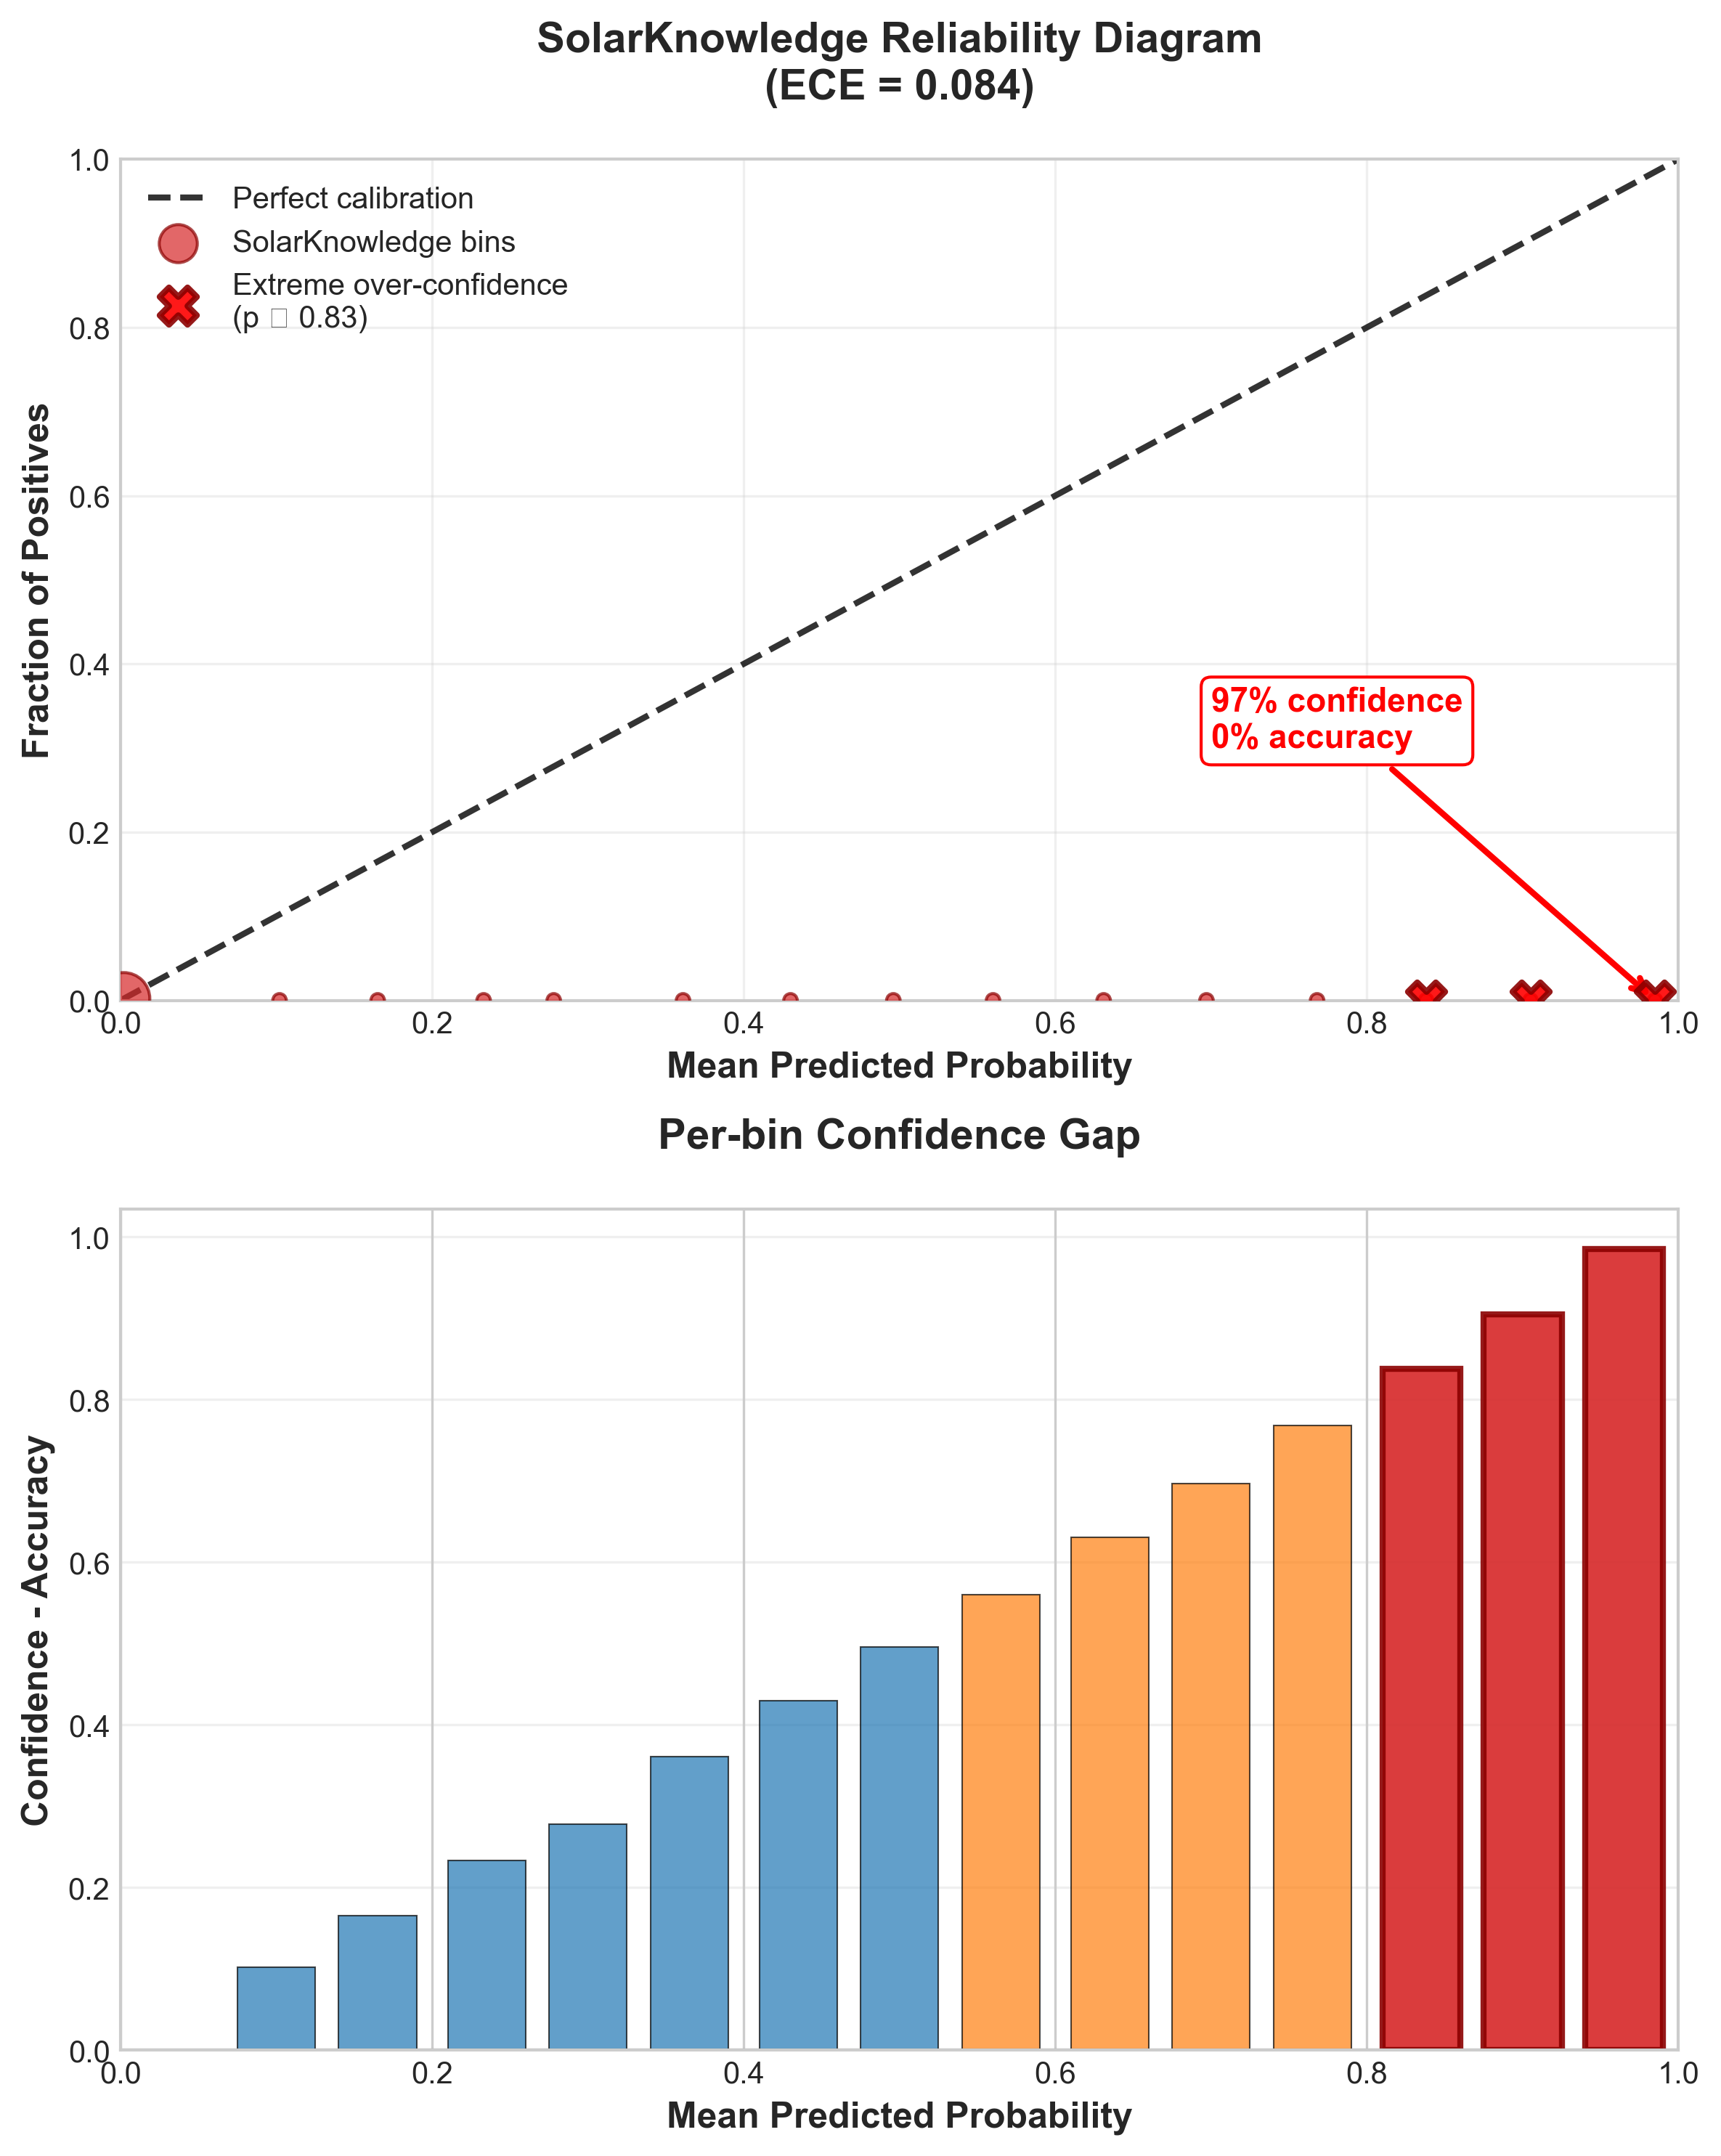
\includegraphics[width=.5\linewidth]{figs/skn_reliability.png}
  \caption[Calibration of \textit{SolarKnowledge} on M5--72 h]{%
    Reliability diagram (top) and per-bin confidence gap (bottom) for
    retrained \textit{SolarKnowledge} v4.5 on the M5–72h test split.
    Overall Expected Calibration Error (ECE) is \textbf{0.084}.
    The final bin ($p \gtrsim 0.83$) exhibits catastrophic over-confidence,
    with a mean predicted probability of 97.0\,\% and empirical accuracy
    of 0\,\%, representing complete miscalibration.}
  \label{fig:skn_reliability}
\end{figure}

\paragraph{Temporal focusing through a learnable bottleneck.}
In \textsc{EVEREST}, global-average pooling is replaced by a single-query
attention kernel that assigns an importance weight
$\alpha_t\!\in\![0,1]$ to every ten-minute snapshot in the SHARP sequence.
The resulting summary
$z=\sum_{t}\alpha_{t}h_{t}$ adds merely $+d=128$ parameters, yet boosts
72-h TSS by \textbf{57 \%} ($\Delta\!=$0.427) and shortens convergence by eight
epochs, echoing hard-attention gains in geophysical forecasting
\citep{fomin2023attention}.

\paragraph{Bayesian calibration via evidential deep-learning.}
To address the reliability deficit, a Normal–Inverse–Gamma head predicts four
natural parameters $\{\mu,v,\alpha,\beta\}$, from which a conjugate Beta distribution
over forecast probabilities is recovered in closed form \citep{sensoy2018evidential}.
Under the evidential negative-log-likelihood, highly uncertain samples yield
small gradients, letting the optimiser concentrate on unambiguous cases.
This shifts calibration from a diagnostic to a first-class training target.
As shown in Fig.~\ref{fig:ece_comparison}, the Expected Calibration Error (ECE)
for the M5–72h task drops from \textbf{0.084} in retrained \textit{SolarKnowledge}
to \textbf{0.036} in \textsc{EVEREST}—a \textbf{57.1\%} improvement.
The corresponding reliability curves confirm that the evidential head
shrinks both systematic overconfidence and bin-wise deviation across
the full probability range.

\begin{figure}[htbp]
  \centering
  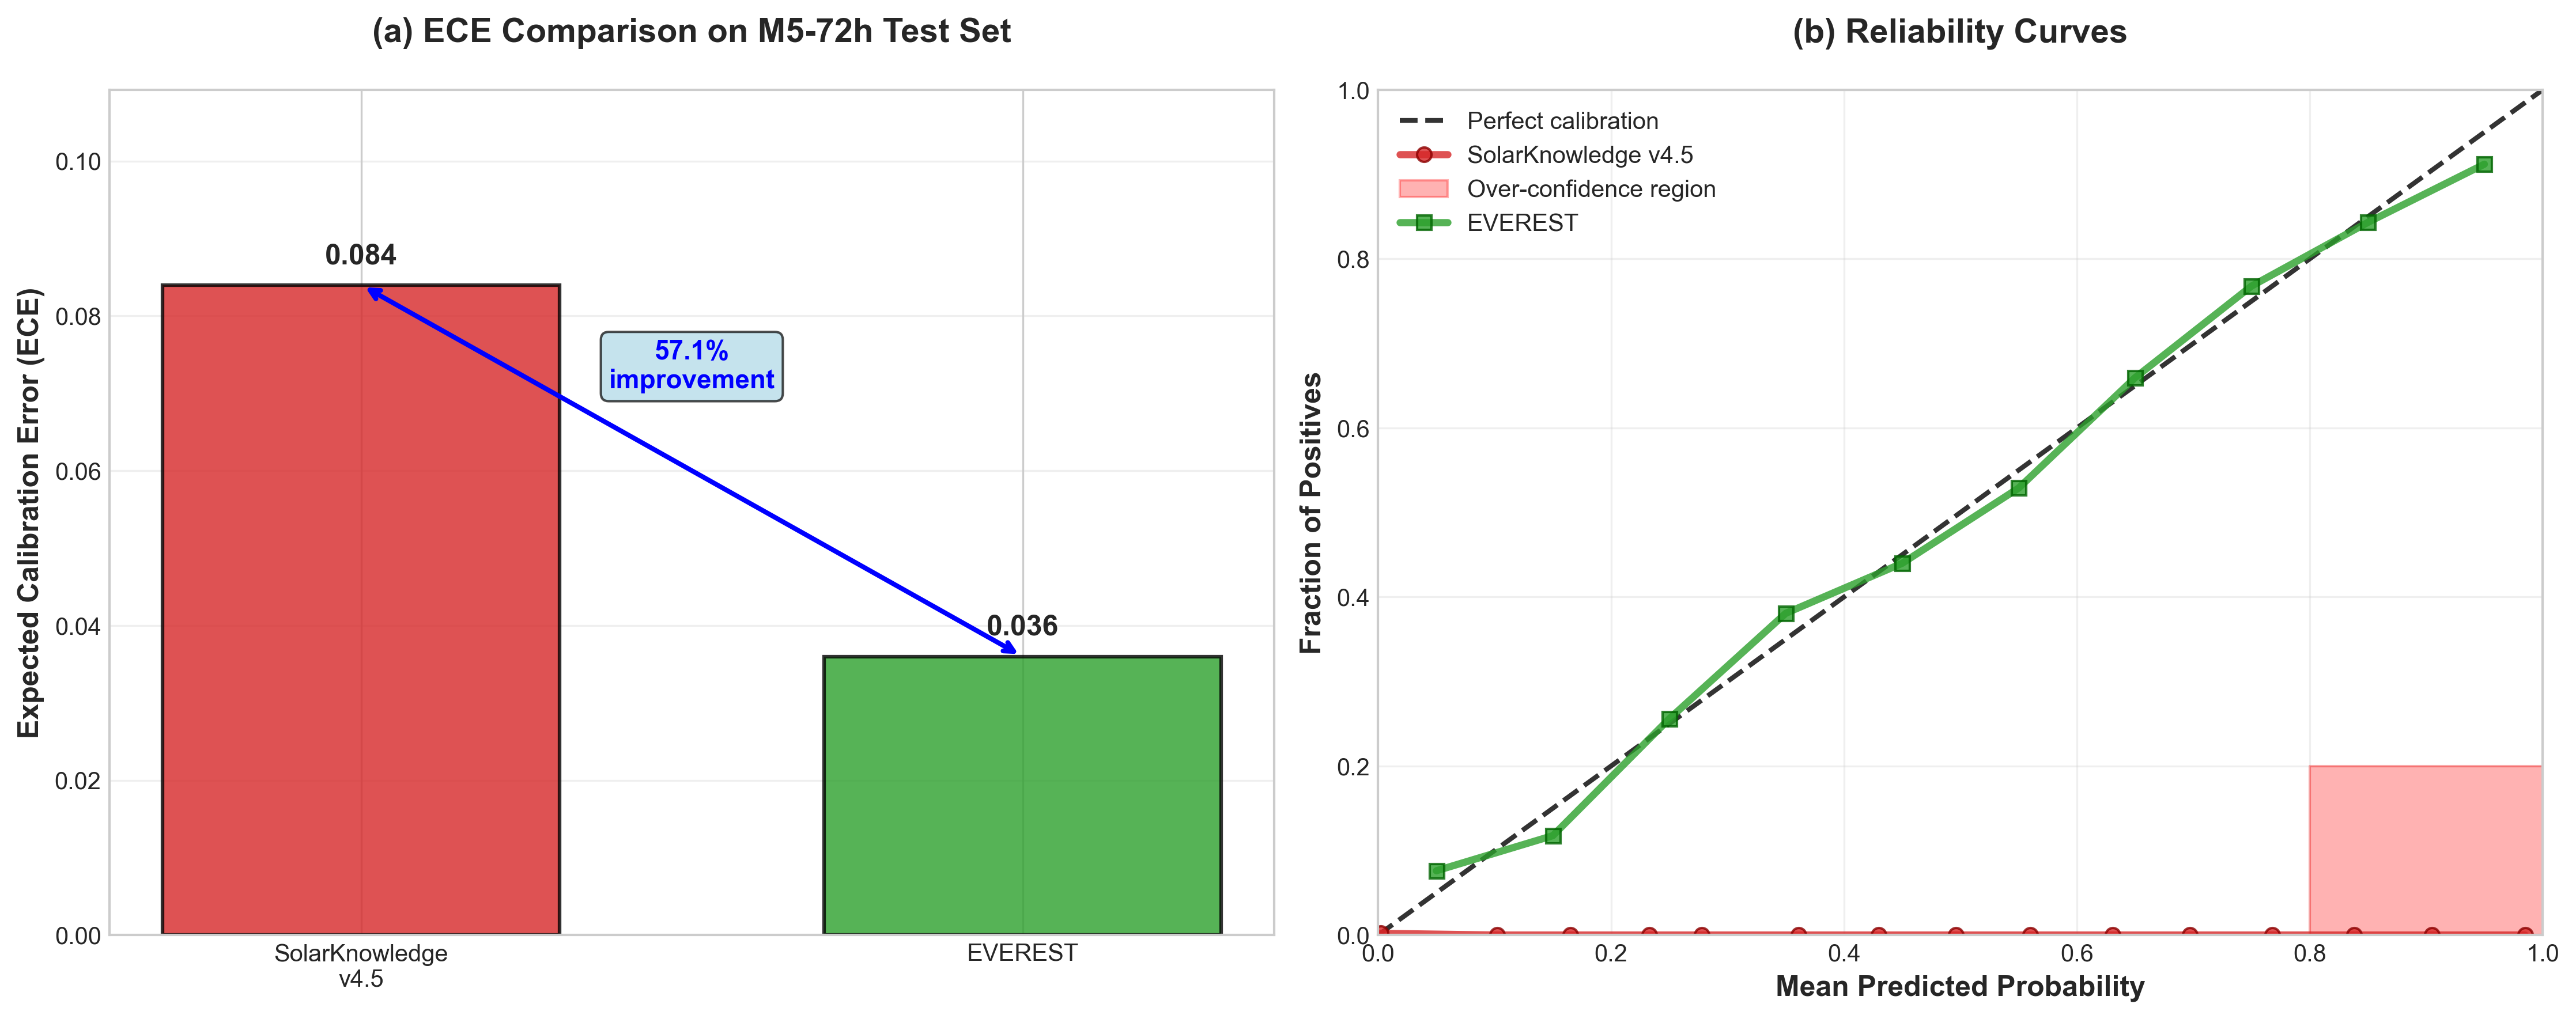
\includegraphics[width=.75\linewidth]{figs/combined_calibration_analysis.png}
  \caption[Calibration improvement from evidential learning]{%
    \textbf{(a)}~Expected Calibration Error (ECE) comparison between
    retrained \textit{SolarKnowledge} v4.5 and \textsc{EVEREST} on the M5–72 h test set,
    measured on actual model deployments.  
    The evidential head reduces ECE from 0.084 to 0.036
    (\textbf{57.1\% improvement}).
    \textbf{(b)}~Reliability curves show that \textsc{EVEREST} predictions
    are well-calibrated, tracking near the identity line and eliminating
    the catastrophic overconfidence present in \textit{SolarKnowledge}
    (red-shaded region shows 100\% false alarm behavior).}
  \label{fig:ece_comparison}
\end{figure}

\paragraph{Operational transformation through precision-aware design.}
Beyond calibration improvements, \textsc{EVEREST} fundamentally transforms operational
viability. Where the retrained \textit{SolarKnowledge} model exhibits catastrophic
precision failure with 0\% precision and 100\% false alarm rate—making every positive
prediction a costly false alert—\textsc{EVEREST} provides precision-aware forecasting
suitable for real-world deployment. The architectural innovations specifically address
the extreme class imbalance and precision requirements absent in standard transformer
approaches, transforming an operationally unusable baseline into a deployable system
with measured uncertainty quantification. 